\documentclass[10pt, a4paper]{scrartcl}
\usepackage{a4wide}
\usepackage[utf8]{inputenc}
\usepackage{ngerman}
\usepackage[pdftex]{graphicx}
\usepackage{floatflt}
\usepackage{float}
\usepackage{wrapfig}



\title{Miniprojekt Bibliotheksverwaltung \\ \normalsize{Projektdokumentation}}
\author{Thomas Kallenberg, Martin Schwab}

\begin{document}
\maketitle
\section{Codequalität}
\subsection{Repository}
Das Repository wird von einem Hudsonserver überwacht. Zudem gibt es ein lokales Shell-Script welches einen Commit verhindert wenn es Fehler oder Warnungen im Code gibt. Sollte dieses Script umgangen werden um mutmaslich nichtkonformen Code hochzuladen, wird der Verursacher mit der Rechnung eines gemeinsamen Mittagessen im Dieci bestraft! (Maximalwert 30.- SFr)

\subsection{Coding-Styleguide}
Vor jedem Commit wird die Eclipse-Standardformatierung angewendet. Zudem werden die Empfehlungen von Sun (http://java.sun.com/docs/codeconv/html/CodeConvTOC.doc.html) für die Codeformatierung benutzt.

\section{Papier-Prototypen}
Die eingescannten Prototypen befinden sich aus Platzgründen in separaten Dateien im selben Verzeichnis wie dieses Dokument.

\subsection{Prototyp 1 - 09.10.2009}
Pro Aufgabe (Ausleihe, Rückgabe, Verwaltung, Reservation) steht hier ein Button zur Verfügung. Aber: Weiss man schon im Voraus, ob man ein Buch ausleihen oder reservieren will? Muss man es nicht zuerst suchen? Was bedeutet ''Verwaltung'' bzw. was wird verwaltet? Durch die geöffneten Fenster kann das Interface schnell unübersichtlich werden.

\subsection{Prototyp 2 - 11.10.2009}
Mit dem minimalistischen GUI konnten die Muss-Kriterien nicht erfüllt werden. Die Undo-History auf der rechten Seite lässt sich nur schwer realisieren. Da die Aktionen voneinander abhängig sein können, würde der Aufwand für die Implementation zu komplex. Das Menü links deckt zudem nicht alle Muss-Kriterien ab.

\subsection{Prototyp 3 - 11.10.2009}
Hier stellt sich beim Testen heraus, dass der Text auf dem Button ''Ausleihen'' irreführend ist, da er mit dem Verb ''ausleihen'' verwechselt wird. Der Knopf sollte alle ausgeliehenen Bücher anzeigen und dient nicht dazu, ein neues Buch auszuleihen. Ein weiterer Punkt sind die farbigen Bestätigungen, welche als lästig empfunden werden. Verbesserungsvorschlag: Eingelesene Bücher werden beim einscannen automatisch ausgeliehen / zurückgegeben und man kann den Vorgang in der Liste rückgängig machen. Statt dem Bestätigungs-Knopf soll ein ''zurück-zum-Hauptfenster''-Knopf angezeigt werden. Als letzter Mangel sei das ''R'' erwähnt, bei welchem nicht gleich klar ist, dass es für ''Reserviert'' stehen sollte. 

\begin{wrapfigure}{r}{45mm}
  \begin{center}
   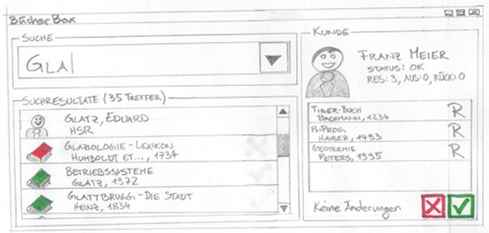
\includegraphics[width=45mm]{prototyp3Thumbnail} \\
   Prot. 3, Benutzeransicht
  \end{center}
\end{wrapfigure}

Und noch etwas: Der Laserscanner funktioniert wie ein normales Eingabegerät. Wird ein Code mit dieser Methode eingelesen, sollte dieser nicht an das Ende des Suchtextes angehängt werden. Ist man im Ausleihemodus, sollte der Suchtext unverändert bleiben, wenn man einen Buchcode einscannt.

\subsection{Prototyp 4 - 14.10.2009} 
\begin{wrapfigure}{r}{45mm}
  \begin{center}
   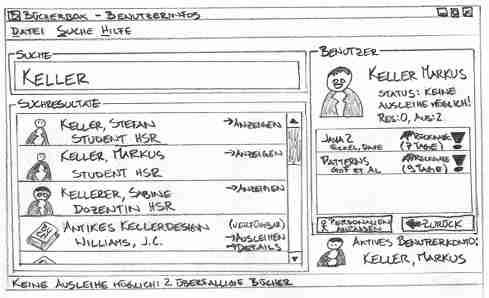
\includegraphics{prototyp4Thumbnail} \\
   Prot. 4, Benutzer mit Mahnungen
  \end{center}
\end{wrapfigure}
Auf das Feedback eines Projektbetreuers hin, dass der Status des Systemes nicht gut sichtbar ist, wurde in der rechten unteren Ecke ein Informationsfeld hinzugefügt, welches den zur Zeit aktiven Benutzer anzeigt. Das Kuchendiagramm auf dem Hauptbildschirm, welches über den Zustand der Bibliothek informiert wurde entfernt, da nicht interessant im täglichen Gebrauch. Neu ist zudem die Menüleiste, welche den Lernprozess unterstützen soll.

Ein weiterer Nebenprototyp wurde verworfen. Es wurde versucht, im unteren Teil des Userinterfaces eine Detailanzeige einzufügen, so dass das Fenster zu einem Quadrat wurde. Dies hätte jedoch die Übersichtlichkeit der Benutzeroberfläche beeinträchtigt und zudem sind moderne Bildschirme eher breit als hoch.

\subsection{Prototyp 5 - 15.10.2009}
\begin{wrapfigure}{r}{45mm}
  \begin{center}
   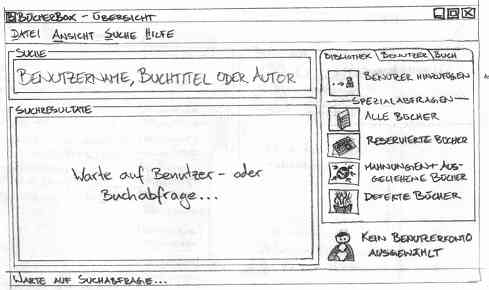
\includegraphics{prototyp5Thumbnail} \\
   Prot. 5, Übersicht
  \end{center}
\end{wrapfigure}
Der gestrige Prototyp wurde heute von einer echten Bibliothekarin der HSR getestet. Das Feedback ist in diesen neuen Prototypen eingeflossen. Verschiedene Beschriftungen wurden entfernt oder aus Verständlichkeitsgründen geändert. Es stellt sich heraus, dass die ''Zurück''-Buttons nicht verständlich sind. 
Als Gegenmassnahme wurden auf der rechten Seite Tabs eingeführt, welche über das aktuell ausgewählte Buch oder den letzten Benutzer Details anzeigen und es ermöglichen, wieder ins Hauptmenü zurückzukehren.

Interessant war ebenfalls, dass das produktive System der HSR-Bibliothek die Bücher beim Einscannen ohne weiteres Nachfragen zurückbucht. Das Vorgehen ist deshalb gefahrlos, da die Bibliothekarin das Buch ja in den Händen hält, es sich somit in der Bibliothek befindet. Der Klickaufwand wird so enorm minimiert. Es wird versucht, diesen Ablauf in das Miniprojekt einzubauen, wenn eine Bücher-ID gescannt oder getippt wird. Für Demonstrationszwecke wird es trotzdem nötig sein, dass man nach einem Buchtitel suchen kann und diesen ausleihen oder reservieren kann.

\subsection{Prototyp 6 - 16.10.2009}
\begin{wrapfigure}{r}{45mm}
  \begin{center}
   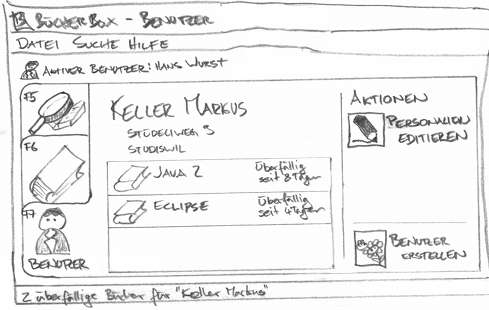
\includegraphics{prototyp6Thumbnail} \\
   Prot. 6, Benutzeransicht
  \end{center}
\end{wrapfigure}
Der Projektbetreuer hält folgende Punkte fest: Der Status des aktiven Benutzers ist zu wichtig, um ihn in die rechte untere Ecke zu drängen. Besser wäre, ihn rechts oder links oben zu platzieren. Zudem sind die Tabs auf der rechten Seite klein, um alle wichtigen Aktionen darin ausführen zu können. 
Während des Gesprächs hat sich herausgestellt, dass das Suchfenster ohne weiteres in einen Tab ausgelagert werden könnte. Damit wäre das Platzproblem für die Aktionen gelöst. 

Der neue Prototyp hat immer noch 3 Tabs, die jetzt auf der linken Seite platziert und mit einem Bild und einem Accelerator versehen wurden. Der ''Bibliothek''-Tab wurde umgewandelt in einen ''Recherche''-Tab und die Spezialsuchabfragen sind in einer Spalte auf der rechten Seite aufgelistet. Am linken oberen Rand des Fensters prangt neu das Feld mit dem aktiven Benutzer. Eine Schwierigkeit wird jetzt sein, den Übergang von der Recherche zu den Buchdetails mit möglichst wenig Aufwand zu gestalten.

\subsubsection{Review 23.10.2009}
Dank dem Review konnten drei weitere Punkte verbessert werden. Das ''X''-Bild beim defekten Buch sieht aus wie ein Button. Er wird deshalb ersetzt durch ein Durchstreichen des Buchtitels und einem kleineren Kreuz-Symbol neben dem Text zum Zustand. Als zweites war das zur Zeit gewählte Buch nicht ersichtlich, weshalb bei der TabbedPane ein ToolTip eingeblendet wird mit dem Titel des ausgewählten Buches. Zuletzt sollten im ''Aktionen''-Bereich mehr Knöpfe vorhanden sein, wie zum Beispiel ''Buch suchen'' oder ''Neue Suchanfrage''.

\end{document}






